\chapter{Analýza požadavků a cílů}
\label{chap:analysis}
Jelikož jednoduchá správa reklamních kampaní je problém existující delší dobu, existují nástroje ulehčující tuto úlohu. Aby bylo jasné, jak
je možné ulehčit a zrychlit tvorbu těchto kampaní, je potřeba se seznámit s tím, co všechno taková tvorba obnáší.
Tato kapitola se zmiňuje o potřebách při vytváření různých druhů reklamních kampaní, porovnává několik vytvořených nabízených
nástrojů na řešení správy kampaní.

\section{Reklamní kampaně}
Reklamní kampaň lze definovat jako soubor komunikačních a reklamních aktivit, které mají za úkol oslovit veřejnost a splnit zvolený cíl. K uskutečnění kampaně se dá využít různých komunikačních
médií (internet, rozhlas, televize, \ldots). Pokud má být reklamní kampaň úspěšná, měla by být promyšlená. Tento úkol dokáže usnadnit úvaha nad následujícími body.


\subsection{Cíl kampaně}
Zvolení cíle zavisí na tom, co chceme kampaní dosáhnout. Typicky se jedná o zvýšení prodejnosti zboží nebo služeb, to ale nejsou jediné možnosti. Další mohou být například budování
povědomí o své značce (brand) nebo předání nějaké informace. Znát cíl pomáhá s další tvorbou kampaně a udává její směr.

\subsection{Rozpočet}
Finanční možnosti jsou jedním ze základních kritérií, ne-li nejdůležitějším. Od rozpočtu se odvíjí nejen celý zbytek plánování reklamní kampaně, ale i možná
doba trvání kampaně. Je velice pravděpodobné, že malý rozpočet se rychleji vyčerpe a proto je nutné kampaň vhodně rozložit.

\subsection{Publikum}
Cílové publikum je další důležitý faktor. Tato volba může znamenat rozdíl mezi dobrou nebo špatnou investicí. Různá sociodemografická kritéria pomohou lépe porozumět
na koho se kampaň směřuje. Toho lze využít při vytváření plánů komunikace, reklamy, nebo volby média.

\subsection{Média}
Různá média, různě působí na zvolené cílové publikum. I proto je dobře specifikované cílové publikum důležité. Pokud je cilovým publikem například starší populace, investice
do PPC reklamy může být značně nevýhodná. Dalším kritériem pro výběr komunikačního kanálů mohou být možnosti geologického cílení, zpětné vazby a statisky úspěšnosti.
S výběrem správného média může pomoct tzv. \emph{Afinita}. Afinita je index určující vhodnost reklamního nosiče, vyjádřená jako poměr sledovanosti média cílovým publikem
a obecné populace. Čím vyšší afinita, tím vyšší možnost oslovení cílového publika.

\subsection{Soudržná komunikace}
Posledníl, neméně důležitá podmínka pro úšpěšnou kampaň, je soudržná prezentace brandu
\footnote{Brand označuje značku organice, výrobku nebo služby. Pod brandem je myšleno jak grafické vyjádření, tak i podstata toho, co znázorňuje.}
nebo promovaného zboží. Dobrá komunikace vede k lepšímu rozpoznání potenciálním zákazníkem a zdůrazňuje, že zde je zákazník na správném místě.

\section{Internetové kampaně}
Různé studie neustále poukazují na čím dál více se zvyšující čas jednotlivcem strávený na Internetu. Pro spoustu inzerentů to znamená vyšší možnost
zaujmutí zákazníka a celkově větší možné publikum. Internet se tímto stal velice atraktivním médiem a to nejen díky vysoké míře \emph{OTS}
\footnote{Opportunity to see, průměrná možnost zhlédnutí reklamy příslušníkem cílového publika během kampaně.},
ale také jednoduché možnosti cílení a monitorování úspěšnosti reklamy.


\subsection{Poskytované typy sítí}
Pro spoustu uživatelů Internetu se jejich pomyslnou bránou do tohoto digitálního světa staly vyhledávače. Není divu, že se tyto vyhledávače staly jedním z největších
poskytovalů online reklamy. Z toho plyne i první typ reklamní sítě. A tou je právě \emph{Vyhledávácí síť}. Reklama zde bývá zobrazena ve formě textových odkazů,
vedoucí na webové stránky inzerenta. Ač se jedná o jednoduchou a negrafickou reklamu, jedná se o jednu z nejúspěšnějích forem reklamy, co se prokliků týče. Tato skutečnost
je způsobena tím, že se uživateli zobrazují výsledky spojené s tím, co si zahledal, tedy pro něj mají vysokou relevanci.

Dalším typem jsou \emph{Obsahové sítě}. Jedná se většinou o sdružení partnerských webů, které se snaží o jednotnou identifikaci uživatele. Reklama na síti tohoto typu bývá
grafická, ve formě bannerů, videoreklamy, nebo celostránkové reklamy\footnote{Sklik tyto možnost nabízí pod názvem \enquote{Branding}}.

Jako třetí typ se autor rozhodl uvést také \emph{Sociální sítě}. Ty na základě zájmů svých uživatelů, sociálních grafů a podobných technik nabízejí dobře cílenou inzerci.
Ta může být grafická a zároveň interaktivní. Nejčastějším trendem je reklama vložená do tzv. \enquote{stories}.

\subsection{Typy kampaní}
Typy kampaní jsou závislé na systému, které je poskytuje. Typicky ale lze očekávat podporu například videokampaní, obsahových kampaní nebo taky produktové kampaně.
Typy kampaně ovlivňuje, kde se bude reklama zobrazovat a jaké formáty podporuje. Zajímavým typem kampaně je produktová kampaň. Zatímco ostatní kampaně mají
pevně\footnote{Textace, bannery apod. se ručně nastavují} nastaveny parametry reklamy, produktové kampaně získavají data z tzv. XML feedů. 

\subsubsection{XML feed}
Jedná se o datový soubor v XML formátů popisující nabízené položky zboží. Tento soubor se dá vytvořit ručně, ale mnoho moderních e-shopových řešení
s tímto počítají a umí ho automaticky generovat. Soubor musí být dostupný na veřejném URL. Jakmile je toto splněno, reklamní systémy a taky například
srovnávače zboží si mohou tento feed stáhnout a zpracovat. K onomu stáhování dochází periodicky, v případě změn dat. Časové rozestupy si cílový systém
volí sám. To s sebou přínáší jednu nevýhodu v podobě dostupnosti zboží. Může se stát, že e-shopu dojde zboží na skladě, ale dokud si reklamní systém
nestáhne nový feed, bude nabízet zboží, které není na skladě.

Výhoda XML feedu je v tom, že jeho struktura je dobře strojově čitelná a dá se upravovat. Jeden feed se tedy dá upravit tak, aby pasoval do více
cílových systémů. Dále se také mohou provádět různé optimalizace a úpravy, např. změna ceny zboží v závislosti na konkurenci nebo třeba úprava produktových náhledů.

\subsection{Cílení pomocí cookies}
Ve velké většině připadů inzerentní služby získávaly data o návštěvnících různých webových stránek pomocí cookies třetích stran. Tedy cookies, které
jsou zapsány z jiné domény, než navštívené. 
\begin{figure}[h]
    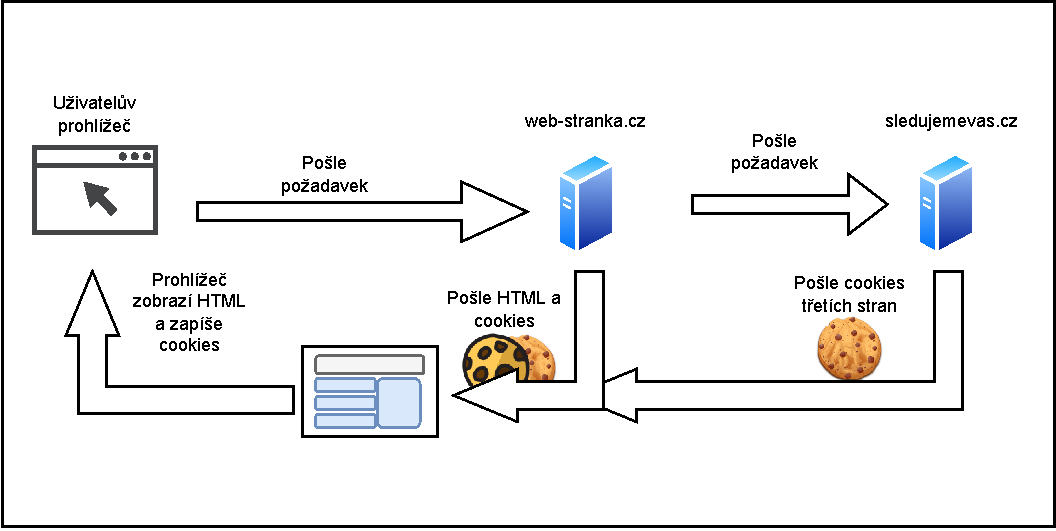
\includegraphics[width=1.0\textwidth]{Figures/cookies.drawio.pdf}
    \caption{Cookies třetích stran}
    \label{fig:cookies}
\end{figure}
Nové směrnice EU, které vynucují lepší ochranu soukromí uživatelů, donutily webové prohlížeče, aby tyto cookies třetích stran zakázali, čím se sledování
návštěvníků omezí. Jedna z možností řešení tohoto problému pro inzerenty je registrace/přihlášení uživatele na daném webu pomocí jiné platformy, známo pod protokolem
OAuth 2.0.

\section{Existující nástroje pro tvorbu kampaní}

\subsection{Sklik}
Český Sklik provozuje svůj systém ve formě webové aplikace. Nabízí import a export kampaní 
(ve formátu CSV\footnote{Ačkoliv formát naznačuje oddělení polí čárkami, ve skutečnosti jedná spíše o znak tábulátoru.})
pro zálohování nebo přenos mezi dalšími systémy. Takto exportovaný soubor má výhodu přímé a rychlé editace dat, ale je podmíněn nutnou znalostí významu jednotlivých
sloupců. Při importu je možné využít nastavení pro přepočet měny, najít a nahradit, filtr na určité sloupce a typ import, tedy zda má import kampaně přepsat, aktualizovat
nebo duplikovat.
Další funkcí jsou návrhy klíčových slov. Tato funkce uživateli zobrazí hledanost klíčového slova (počet zahledání za období), roční trend, velikost konkurence a průměrnou
cenu za proklik reklamy zobrazenou na dané klíčové slovo. Poslední a velice užitečná funkce jsou automatická pravidla. Automatická pravidla se mohou nastavit buďto na
celé sestavy nebo jednotlivá klíčová slova. Jejich účel je automatické zvyšování/snižování ceny za proklik na zákládě například: počtu prokliků, zobrazení konverze, atd.
Tímto dynamickým ovládáním ceny za reklamu si inzerenti mohou v případě dobré výkonnosti sestavy/klíčového posílit svou pozici oproti konkurenci, nebo snížit náklady
v případě, kdy se nedaří.


\subsection{Google Ads Editor}
Nástroj vytvořený společností Google je desktopová aplikace s možností správy nejen kampaní, ale také inzerentních účtů na platformě Google Ads. Využitím operace
\emph{drag and drop} lze jednoduše kopírovat sestavy a kampaně a další nastavení. Při vytváření kampaní může uživatel zadat nebo vybrat nesprávné kombinace určitých
nastavení, je však na ně ihned upozorněn a nucen je opravit. Pro nastavení ceny nabídek se namísto automatických pravidel,
uplatňuje tzv. \emph{strategie nabídek} (angl. Bid strategy). Zde uživatel může vybrat pevně danou cenu za proklik, nebo strategii na maximalizaci prokliků, konverzí
a další. Těmto strategiím se dají nastavit stropní hodnoty. Dalším zajimavým nastavením je také rotování reklam, tedy jak často se budou zobrazovat reklamy v této
kampani, podle toho, jak se jim daří. Většina ostatních nastavení lze rychle vyplnit a vytvořit sestavy a reklamy.

\subsection{Mergado}
Produktové kampaně využivají primárně data z XML feedu. Často se však stává, že je potřeba ve feedu udělat udělat nějaké úpravy, validovat správnou strukturu nebo feed
optimalizovat. Platforma Mergado umožňuje provádět tyto změny v XML feedu z prostředí prohlížeče bez jakéhokoli zásahu programátora. Tento upravený feed je poté
poslán na srovnávače zboží (Heureka, Zboží.cz, \ldots), případně na inzerentní systémy jako například Sklik. Mergado přes svůj \emph{App Cloud} umožňuje například
upravení cen produktů v XML v feedu v závislosti na ceně konkurentů, automatickou úpravu biddingu nebo dokonce obrázkovou úpravu produktovýchg náhledů.

\subsection{XeMeL}
Další nástroj pro úpravu XML feedů. Mezi jeho silné stránky spadá to, že XML feedy aktualizuje každých 45 minut, dokáže spojit více feedů do jednoho, případně
se přizpůsobí i na odlišené vstupní feedy.

\section{Požadavky na vlastní nástroj}
% TODO: Zmínit možnosti editace kampaní - proč je CSV lepší než klikat na webovce

\subsection{Tvorba kampaní}
Možnost tvorby kampaní se může rozložit buďto na jednolivé systémy nebo vytvořením "Super kampaně." Super kampaň bude mít možnost rozložení mezi více platforem pro správu kampaní.
Pro každý z těchto systémů budou různé možnosti nastavení parametrů kampaně, podle podpory funkcí na daném systému. Příkladem může být nastavení denní rozpočtu, geologické cílení atd.
Výhodou takové nastavení bude maximální kontrola nad kampaněmi, ale všechny potřebné věci (bannery, klíčová slova a další) budou spravovány na jednom jednoduchém rozhraní.

\subsection{Import a export}
Možnost importovat a exportovat kampaně je nutný základ pro možnosti správy. Nejčastější formát pro import a export je textový soubor CSV. Struktura se obecně ve více inzerentních
systémů příliš neliší, ale mohou nastat nějaké drobné odchylky\footnote{\href{https://support.google.com/google-ads/editor/answer/57747}{https://support.google.com/google-ads/editor/answer/57747}}
nebo alternativní názvy, se kterými je nutné si poradit. Dále je správný export podmíněm tím, že každý řádek musí popisovat samostatnou položku kampaně.
Jakmile je toto vyřešeno, je možné importovat kampaně a naopak exportovat a následně nahrávat do víceméně každého reklamního systému.

\subsection{Správa a editace kampaní}
Pro správu a editaci existuje spousta nástrojů. Z hlediska efektivity práce je jedna z nejrychlejších cest tvorby kampaní použití tabulkových procesorů. Tabulkové procesory
umožnují rychlou editaci v podobně duplikace a úprav hodnot pomocí klávesnice bez nutnosti neustálého proklikávání myší. Naopak zase neumožňují například validaci
zadaných dat, návrhy klíčových slov a ostatní služby. Výše popsané nástroje jsou velice závislé na uživatelském rozhraní a neumožňují jednoduchou navigaci klávesnicí.
Nachází se zde potenciál pro vytvoření systémů, kde správa a editace kombinuje výhody rychlé a jednoduché navigace s využitím klávesnice a přitom uživateli validatovat
zadávané hodnoty. Existuje taky možnost napojení na API dalších stran a získat další informace, např. návrhy klíčových slov.

\subsection{Úprava XML Feedu}

\endinput